\documentclass{standalone}

\usepackage[usenames,dvipsnames]{xcolor}
\usepackage{tikz}
\usepackage{pgfplots}
\usepackage{graphicx}

\pgfplotsset{compat=newest}

\definecolor{IBM1}{HTML}{648fff}
\definecolor{IBM2}{HTML}{785ef0}
\definecolor{IBM3}{HTML}{dc267f}
\definecolor{IBM4}{HTML}{fe6100}
\definecolor{IBM5}{HTML}{ffb000}
\definecolor{IBM6}{RGB}{051,117,056}

\definecolor{Okabe1}{RGB}{000,158,115}
\definecolor{Okabe2}{RGB}{000,114,178}
\definecolor{Okabe3}{RGB}{086,180,233}
\definecolor{Okabe4}{RGB}{230,159,000}
\definecolor{Okabe5}{RGB}{213,094,000}
\definecolor{Okabe6}{RGB}{204,121,167}

\usepackage{pgfplots,pgfplotstable}
\usetikzlibrary{positioning}

%\pgfplotstableread{
%	X Y  
%	-3  9  
%	-2  7  
%	-1 5  
%	0 3  
%	1 1  
%	2 -1 
%	3 -3
%}\mydata

\usepackage{booktabs}

%\pgfplotstableset{every head row/.style={before row=\toprule,after row=\midrule}, every last row/.style={after row=\bottomrule}}


\begin{document}
		\begin{tikzpicture}[baseline]
		\begin{axis}[
			anchor=center,
			name=myplot,
			legend style={at={(0.025,0.975)}, anchor=north west},
			enlargelimits=false,
			tick pos=left, %
			tick align=outside, %
			axis line style={opacity=0}, %
			title={$b.$},
			title style={yshift=-2ex, xshift=-32ex},
			after end axis/.code={
				\draw ({rel axis cs:0,0}
				-|{axis cs:0,0}) % xmin (line starts here)
				-- ({rel axis cs:0,0}
				-|{axis cs:25,0}); % xmax (line stops here)
				\draw ({rel axis cs:0,0}
				|-{axis cs:0,0}) % ymin (line starts here)
				-- ({rel axis cs:0,0}
				|-{axis cs:0,0.3}); % ymax (line stops here)
			},
			xlabel={$p_i$ (kPa)},
			ylabel={$c$},
			xmin=-1.25, xmax=25,
			scaled x ticks=false,
			ymin=-0.01, ymax=0.3,
			scatter/classes={
				%c={mark=*,color=Okabe5},
				b={mark=*,color=Okabe1},
				a={mark=*,color=Okabe4},
				d={mark=*,color=gray}
			}
			]
			\addplot[scatter,only marks,% 
			scatter src=explicit symbolic % Needed for scatter class styling
			] 
			table[meta=label] {
				x y label
				0	0	d
				1	0.015549598	a
				2	0.022520107	a
				3	0.036997319	a
				4	0.044504021	a
				5	0.051474531	a
				10	0.080965147	a
				15	0.105093834	a
				20	0.119034853	a
				25	0.133512064	a
				0	0	d
				1	0.04021164	b
				2	0.061904762	b
				3	0.080952381	b
				4	0.097354497	b
				5	0.108465608	b
				10	0.156613757	b
				15	0.18994709	b
				20	0.215343915	b
				25	0.231746032	b
				%0	0	d
				%1	0.057619817	c
				%2	0.08723748	c
				%3	0.109854604	c
				%4	0.129240711	c
				%5	0.148626817	c
				%10	0.211093161	c
				%15	0.261712439	c
				%20	0.293484114	c
				%25	0.325255789	c
			};
			%\addlegendentry[anchor=west]{0.75 mm}
			\addlegendentry[anchor=west]{$s_g =$ 3.7 mm}
			\addlegendentry[anchor=west]{$s_g =$ 3.2 mm}
			\node[anchor=south east,inner sep=0] at (20,0) {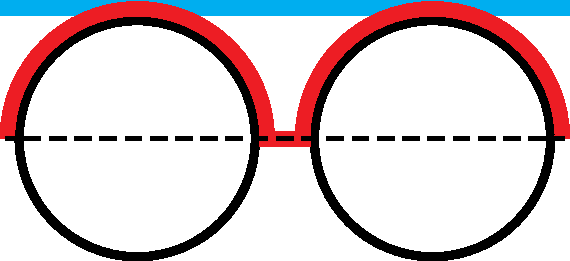
\includegraphics[trim = 0 0 0 0, clip, width=2cm]{GrainConformalitySchematic.pdf}};
			\node [anchor=south west, inner sep=0] at (20.5,0.045) {$c = 0$};
			\node [anchor=south west, inner sep=0] at (20.5,0.02) {$c = 1$};
		\end{axis}
	\end{tikzpicture}
%	\begin{tabular}{c c} 
%		\hline
%		$\phi_0$ & $s_g$ (mm)  \\ \hline
%		0.44 &  0.51  \\
%		0.49 & 0.41  \\
%		0.58 & 0.29  \\
%		0.65 & 0.19  \\
%		0.7 & 0.14  \\
%		0.74 & 0.1  \\
%		0.79 & 0.05  \\ 
%		0.84 & 0.02 \\ \hline
%	\end{tabular}
\end{document}